	In this section, we illustrate our results, by numerical experiments. Taking 
as example Chagas disease, we confirm its extinction and persistence under 
real literature parameters. Also we expose how noise perturbation affect our 
deterministic base dynamics under specific functional responses. 

	Chagas disease resides in multiple hosts ---more than \num{100} 
species of mammals \cite{Crawford2014}, including humans and more than one 
vector species \cite{Steverding2014}.  A human can get the disease via bite of 
infected bug, blood transfusion, organ transplantation, ingestion of
contaminated food, vertical transmission and accidental laboratory exposure 
\citep{Nunes2013}. So, for our experiments, we consider humans and one animal 
specie as hosts. For vectors, we use entomological information of 
<<<<<<< Updated upstream
\textit{Triatoma infestans} and since the main 
transmission route of Chagas disease is via bite of infected bug 
\citep{Nouvellet2015}, we only consider this. Also, we put environmental noise 
in this kind of transmission, to be precise, we perturb vector bitting 
parameters 
$z_h$, $z_a$ as in \Cref{sec:sto_ext} with  noise intensities
=======
\textit{Triatoma infestans}. 
Since the main transmission route of Chagas infection is vectorial 
\citep{Nouvellet2015}, we put environmental noise in this kind of transmission.
To be precise, we perturb Triatoma vector bitting parameters $z_h$, $z_a$ as 
in \Cref{sec:sto_ext} with  noise intensities
>>>>>>> Stashed changes
\begin{align}
	F_{1}(I_{h},I_{a},S_{v},I_{v}) 
		= 
		\frac{
			\sigma_{z_h}	H
				}
				{
					K
				}
				I_{v} ,
				&&
	F_{2}(I_{h},I_{a},S_{v},I_{v}) 
		= \frac{
				\sigma_{z_a} A 
			}
			{
				K
			} I_{v} ~.
\end{align}
Hence, our SDE model \eqref{eq.2} becomes
\begin{equation}\label{eq.8}
		\begin{aligned}
			dI_{h} &= 
				\left[
					\alpha_{h}I_{v} 
					\left(
						H-I_{h}
					\right)
					-
					\mu_{h} I_{h}
				\right]dt 
				+\sigma_{z_h} 
				\left(
					\frac{\theta_{h} H}{K}
				\right)
				I_{v}^2 \left( H-I_{h}\right) dW_{1}(t)\\
			dI_{a} &= 
				\left[
					\alpha_{a} I_{v}
					\left(
						A-I_{a}
					\right)
					-
					\mu_{a} I_{a}
				\right]dt 
				+ 
				\sigma_{z_a}
				\left(
					\frac{\theta_{a} A }{K}
				\right)
				I_{v}^2
				\left(
					A-I_{a}
				\right)dW_{2}(t)
			\\
			dS_{v} &= 
				\left[
					\Lambda_{v}
					T_{v}-
					\left(
						\alpha_{v_{h}}I_{h}
						+\alpha_{v_{a}} I_{a} 
					\right) S_{v}
					-
					\left(
						\mu_{v}+r_{K}T_{v} 
					\right) S_{v}
				\right]
				dt 
			\\
<<<<<<< Updated upstream
			&\quad -
			\sigma_{z_h}
=======
			&-
			\psi_{1}
>>>>>>> Stashed changes
			\left(
				\frac{\theta_{v_{h}} H}{K}
			\right)
			 I_{h} I_{v} S_{v} dW_{1}(t)
			-
			\sigma_{z_a}
			\left(
				\frac{ \theta_{v_{a}} A}{K}
			\right)
			I_{a} I_{v} S_{v} dW_{2}(t)
			\\
			dI_{v} &= 
			\left[
				\left(
					\alpha_{v_{h}} I_{h}
					+
					\alpha_{v_{a}} I_{a}
				\right)
				S_{v}
				-
				\left(
					\mu_{v}+r_{K}T_{v}
				\right) I_{v}
			\right] dt 
			\\
<<<<<<< Updated upstream
			&\quad +
			\sigma_{z_h}
=======
			&+
			\psi_{1}
>>>>>>> Stashed changes
			\left(
				\frac{\theta_{v_{h}} H}{K}
			\right)
			I_{h} I_{v} S_{v} dW_{1}(t)
			+
			\sigma_{z_a}
			\left(
				\frac{ \theta_{v_{a}} A}{K}
			\right)
			I_{a} I_{v} S_{v} dW_{2}(t)
				~.
		\end{aligned}
	\end{equation}
<<<<<<< Updated upstream

	As example, we consider a rural community ---~we think in a farmer community 
with less than 10000 habitants as human host population.
Likewise, we assume enough initial infected density to sustain our
different scenarios. So, it is reasonable to consider 
$
	\left(
		I_{h}(0),
		I_{a}(0),
		S_{v}(0),
		I_{v}(0)
	\right) 
	= 
	\left( 
		10,
		50,
		1170,
		30 
	\right)
$ 
as our initial populations. In this way, we illustrate extinction and 
persistence behavior of SDE \eqref{eq.8}, in the context of
\Cref{theo:GSAS,theo:persist}.
Also, we contrast these stochastic scenes with our deterministic base 
($\sigma_{z_h}=0$, $\sigma_{z_a}=0$) dynamics.

Since the coefficients of our model \eqref{eq.8} not satisfies globally, the 
Lipschitz and linear growth conditions, we implement the  Linear-Steklov (LS) 
method reported in \cite{Diaz-Infante2016} ---~see \ref{app:ls_method} for 
details.
=======
\todo{What that fuck with $T_v$?}
	Next, we illustrate extinction and persistence behavior of SDE 
\eqref{eq.8}, in the context of \Cref{theo:GSAS,theo:persist}.
Also, we contrast this stochastic scene with our deterministic base 
dynamics ($\psi_1=0$, $\psi_2=0$). Since the coefficients of our model 
\eqref{eq.8} not satisfies globally, the Lipschitz and linear growth conditions,
we implement the  Linear-Steklov (LS) method reported in 
\cite{Diaz-Infante2016} ---~see \ref{app:ls_method} for details.
%
\todo{numerical method}
\todo{Parameters for the method: step h, resolution, random number generator.}
%
\begin{table}
%	\todo{Format}
	\begin{tabular}{c}
		Initial conditions \\
			\hline
			$I_h = \num{10.0}$		\\
			$I_a = \num{50.0}$		\\
			$S_v = \num{1170.0}$	\\
			$I_v = \num{30.0}$		\\
	\end{tabular}
	\caption{Initial conditions for all experiments.}
\end{table}
%
\subsection{Disease-Free Equilibrium} 
		To numerically show the global stochastic asymptotic stability of 
	disease-free equilibrium point, some parameter values are taken of the 
	literature and are given in~\Cref{table:2}. For the other parameters, we 
	consider that total human and animal population equal to \num{1500} and 
	\num{2500}, 
	respectively; while total maximum allowable number of vectors is equal to 
	$20$ times the total host population. Likewise, we assumed that human and 
	animals lifetime is equal to $70$ and $6$ years, respectively, so 
	$\mu_{h} = \num{0.0142857}$ and $\mu_{a} = \num{0.1666666}$. 
	Finally, with the objective of guarantee the conditions 
	of \Cref{theo:GSAS}, we assumed that $\mu_{v}= \num{281.1}$.
\begin{table}[htb]
	\centering
	\caption{Parameter values of system~\eqref{eq.8} to show the global 
		stochastic asymptotic stability of disease-free equilibrium point
	}\label{table:2}
	\begin{tabular}{cclc}
		\toprule
		Parameters & Value & \multicolumn{1}{c}{Units} & Reference\\
		\midrule
			$z_{h}$ 					& 14.6		&	$\si{bite.year^{-1}.vector^{-1}}$
				&	\cite{Cruz-Pacheco2012a} \\
			$z_{a}$ 					& 40.15		&	$\si{bite.year^{-1}.vector^{-1}}$
				&	\cite{Cruz-Pacheco2012a} \\
			$\tilde{\pi}_{h}$ & 0.0009	&	$\si{human.bite^{-1}}$
				&	\cite{Cohen2001} \\
			$\pi_{h}$ 				& 0.0009	&	$\si{animal.bite^{-1}}$
				&	\cite{Cruz-Pacheco2012a} \\
			$\pi_{v}$ 				& 0.03		&	$\si{vector.bite^{-1}}$
				&	\cite{Cohen2001}				 \\
			$\tilde{\pi}_{v}$ & 0.49		&	$\si{vector.bite^{-1}}$
				&	\cite{Cohen2001}				 \\
			$\Lambda_{v}$ 		& 281.561	&	$\si{year^{-1}}$
				&	\cite{Rabinovich1972}		 \\
			\bottomrule
		\end{tabular}
\end{table}
%
\begin{figure}[!ht]
	\centering
	\subfloat{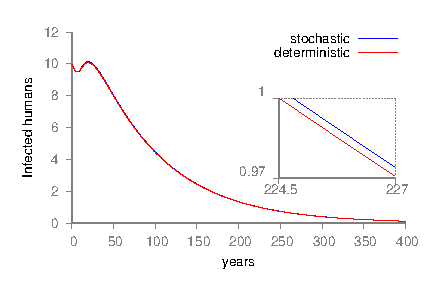
\includegraphics{%
		Sections/Section4/graphs/disease_free/disease_free_infected_humans.eps%
		}
	}
	\subfloat{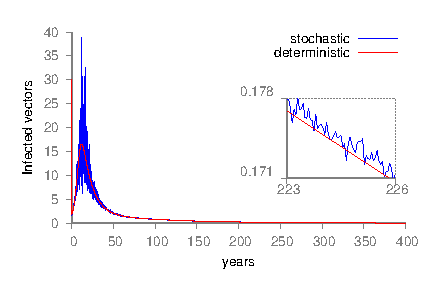
\includegraphics{%
		Sections/Section4/graphs/disease_free/disease_free_infected_vectors.eps%
		}%
	}
	\caption{}\label{Fig.1}
\end{figure}
\begin{figure}[!ht]
	\centering
	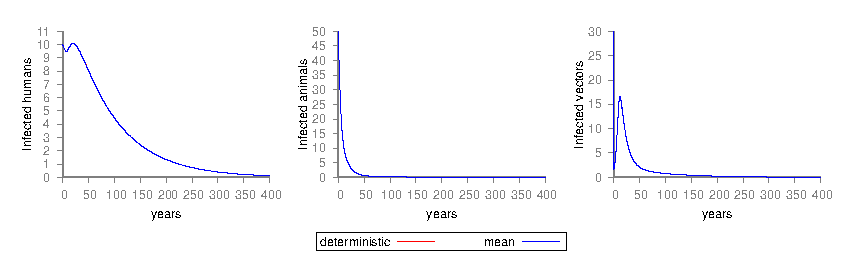
\includegraphics{%
		Sections/Section4/graphs/disease_free/disease_free_mean_population.eps%
		}%
	\caption{}\label{Fig.2}
\end{figure}
\begin{figure}[!ht]
	\centering
	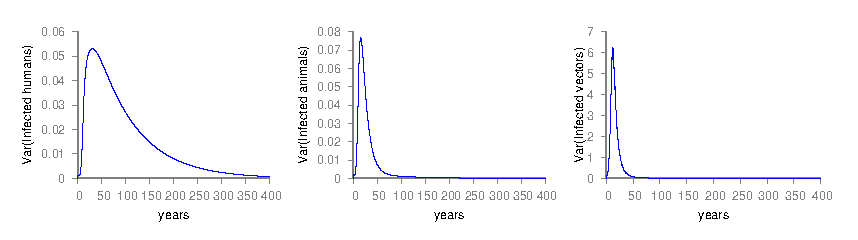
\includegraphics{%
		Sections/Section4/graphs/disease_free/disease_free_variance_population.eps%
	}
\caption{}\label{Fig.3}
\end{figure}
\todo{parameters for moment calculations}

%\begin{figure}[!ht]
%	\centering
%	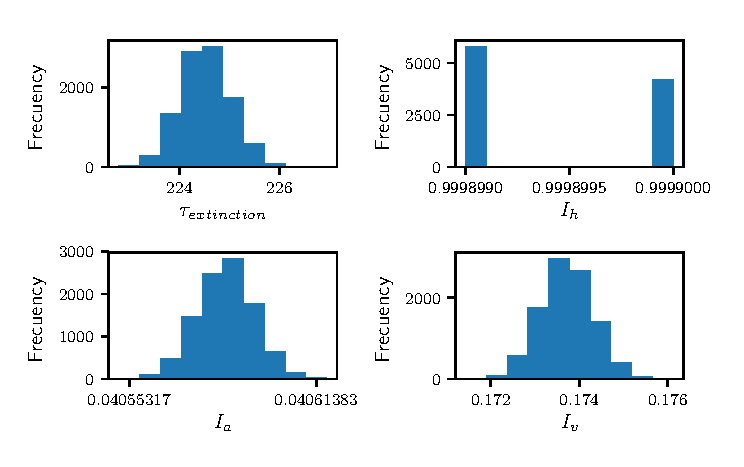
\includegraphics{%
%		Sections/Section4/graphs/disease_free/stopping_time_histograms.eps%
%	}
%\caption{}\label{Fig.3}
%\end{figure}




\subsection{Persistence}
	For guarantee the conditions of \Cref{theo:persist}, we vary the value of 
almost all parameters, thus the total animal population is equal to 
\num[group-separator = {,~}]{3000}, while total maximum allowable number of
 vectors is equal to \num[group-separator = {,~}]{12000}.
On the other hand, for this case, we consider that mortality rate for vectors 
is equal to \num{2.4455} \cite{Rabinovich1972}. The other values are given in 
\Cref{table:3}, while the parameter values that not mentioned are equal that 
in the above case.
>>>>>>> Stashed changes
%
\begin{table}[p]
	\centering
<<<<<<< Updated upstream
	\begin{tabular}{@{}llcll@{}}
		\toprule
		\multicolumn{5}{c}{Set up parameters} 												\\
		\midrule
		\\
		\multicolumn{2}{c}{Initial Conditions} &&
		\multicolumn{2}{c}{Solver Parameters}													\\
		\cmidrule{1-2} \cmidrule{4-5}																	\\
		$I_h(0)=$  \num{10}		&\phantom{abc}&& $h = \num{E-4}$				\\
		$I_a(0)=$  \num{50}		&&& $h_{res}=\num{E-6}$									\\
		$S_v(0)=$  \num{1170}	&&& 																		\\
		$I_v(0)=$  \num{30}		&&& \\
		\bottomrule
	\end{tabular}
	\caption{Set up parameters.}
	\label{tbl:initial_conditions}
=======
	\caption{
			Parameter values of system~\eqref{eq.8} to show 
			persistence
	}\label{table:3}
	\begin{tabular}{@{}crl@{}}
		\toprule
		Parameters & \multicolumn{1}{c}{Value} & \multicolumn{1}{c}{Units} \\
		\midrule
			$z_{h}$ 					& 36.5		&	$\si{bite.year^{-1}.vector^{-1}}$	\\
			$z_{a}$ 					& 182.5		&	$\si{bite.year^{-1}.vector^{-1}}$	\\
			$\tilde{\pi}_{h}$ & 0.002		&	$\si{human.bite^{-1}}$						\\
			$\pi_{h}$ 				& 0.02		&	$\si{animal.bite^{-1}}$						\\
			$\tilde{\pi}_{v}$ & 0.06		&	$\si{vector.bite^{-1}}$						\\
			$\Lambda_{v}$ 		& 2.7			&	$\si{year^{-1}}$									\\
		\bottomrule
		\end{tabular}
>>>>>>> Stashed changes
\end{table}
%